\documentclass[10pt,journal]{IEEEtran}


% *** MISC UTILITY PACKAGES ***
\usepackage[spanish]{babel}
\usepackage[T1]{fontenc}

\usepackage{amsmath,amssymb,amsfonts}
\usepackage{algorithmic}
\usepackage{graphicx}
\usepackage{textcomp}
\usepackage{multirow}
\usepackage{ulem}
\usepackage{booktabs}
%\usepackage[table,xcdraw]{xcolor}
\usepackage[acronym,shortcuts]{glossaries}
\usepackage{pifont}
\usepackage{subcaption}
\usepackage{footnote}
\usepackage{hyperref}
\newcommand{\cmark}{\ding{51}} % Tick (V)
\newcommand{\xmark}{\ding{55}} % Cross (X)
\usepackage{algorithm}
\begin{document}

%
% paper title
% Titles are generally capitalized except for words such as a, an, and, as,
% at, but, by, for, in, nor, of, on, or, the, to and up, which are usually
% not capitalized unless they are the first or last word of the title.
% Linebreaks \\ can be used within to get better formatting as desired.
% Do not put math or special symbols in the title.
\title{Predicción de ataques al corazón :\\ usando Machine Learning }




\author{Jesús Emmanuel Ramos Dávila}







\IEEEtitleabstractindextext{%
\begin{abstract}
Enfermedades cardiovasculares son una de las principales causas de muerte global, con millones de fallecimientos año tras año, Las enfermedades cardiovasculares son un grupo de desórdenes del corazón y los vasos sanguíneos no existe causa exacta para este tipo de enfermedades. Existen algunos patrones de síntomas los cuales están muy asociados a tener este tipo de enfermedades. Actualmente no existen demasiadas investigaciones con respecto a el análisis de grupos y algoritmos de asociación para este tipo de enfermedades.
En esta sección se realizara un estudio usando el algoritmo FCM (Fuzzy C Means) Clustering, para determinar el riesgo de un ataque al corazón, en este estudio se realizara un prueba usando 303 observaciones se revisara el desempeño y la precisión con respecto a otro algoritmo ya conocido.
\end{abstract}

% Note that keywords are not normally used for peerreview papers.
}


% make the title area
\maketitle


% To allow for easy dual compilation without having to reenter the
% abstract/keywords data, the \IEEEtitleabstractindextext text will
% not be used in maketitle, but will appear (i.e., to be "transported")
% here as \IEEEdisplaynontitleabstractindextext when compsoc mode
% is not selected <OR> if conference mode is selected - because compsoc
% conference papers position the abstract like regular (non-compsoc)
% papers do!
\IEEEdisplaynontitleabstractindextext
% \IEEEdisplaynontitleabstractindextext has no effect when using
% compsoc under a non-conference mode.


% For peer review papers, you can put extra information on the cover
% page as needed:
% \ifCLASSOPTIONpeerreview
% \begin{center} \bfseries EDICS Category: 3-BBND \end{center}
% \fi
%
% For peerreview papers, this IEEEtran command inserts a page break and
% creates the second title. It will be ignored for other modes.
\IEEEpeerreviewmaketitle


%\ifCLASSOPTIONcompsoc
%\IEEEraisesectionheading{\section{Introduction}\label{sec:introduction}}
%\else
%\section{Introduction}
%\label{sec:introduction}
%\fi
% Computer Society journal (but not conference!) papers do something unusual
% with the very first section heading (almost always called "Introduction").
% They place it ABOVE the main text! IEEEtran.cls does not automatically do
% this for you, but you can achieve this effect with the provided
% \IEEEraisesectionheading{} command. Note the need to keep any \label that
% is to refer to the section immediately after \section in the above as
% \IEEEraisesectionheading puts \section within a raised box.
\section{Introducción}
\label{sec:introduction}

Enfermedades cardiovasculares son una especie que se están presentando con mayor frecuencia y estas frecuentemente suceden en fallecimientos. La Organización Mundial de la Salud ha estimado alrededor de 12 millones de muertes alrededor del mundo anualmente, debido a este numero avances en la medicina en las últimas décadas habilito la identificación de factores de riesgo que podrían contribuir en este tipo de enfermedades cardiovasculares. La causa más común en este tipo de enfermedades es el estrechamiento o bloqueo de las arterias coronarias. Los vasos que transportan sangre al corazón mismo, Este es llamado enfermedad arteriopatía coronaria y esta sucede comúnmente con el paso del tiempo. Esta es una de las principales causas por las cuales las personas sufren ataques al corazón, Es por eso que un bloqueo que no es tratado dentro de las primeras horas causa que el musculo del corazón muera. Diagnósticos médicos son una importante, pero a la vez una tarea complicada y su automatización podría ser muy útil. Desafortunadamente no todos los doctores están especializados en esta área y no se tiene en algunos casos y no se tienen los mismos recursos médicos. Es por eso que para utilizar el conocimiento de diferentes especialistas y los datos clínicos de pacientes para facilitar el proceso de diagnóstico es considerado muy valioso ya que su integración en tomas de decisiones medicas podría reducir los errores médicos, mejorar la seguridad del paciente y reducir practicas no deseadas.

\section{Metodología}
\label{sec:metodologia}


\subsection{Fuzzy C Means Clustering}

El principal objetivo de esta búsqueda es implementar el algoritmo de Fuzzy C Means Clustering usando nuestros datos de pacientes, esto para poder usarse en el soporte de toma de decisiones, por lo tanto, se desarrolla un modelo Fuzzy C Means para predecir los ataques al corazón.
El algoritmo Fuzzy C-Means Clustering fue desarrollado en 1981 este es un extendido del algoritmo K-Means Clustering,  FCM (Fuzzy C-Means) es un algoritmo no supervisado que es aplicado hacia un rango muy amplio de problemas conectados con análisis de características , clustering y clasificación. FCM también es usado en otros campos además de la medicina, tales como agricultura, ingeniería, astronomía, química, análisis de imágenes.
FCM es una técnica de clustering en la cual un conjunto de datos es agrupado en n-clústeres en la cual cada punto de datos esta relacionado a un clúster el cual tendrá un alto grado de pertenencia hacia este punto siendo así que los puntos de datos que tengan un bajo grado de pertenencia hacia este clúster estarán más alejados de este.

Pasos de algoritmo FCM
\begin{enumerate}
  \item Inicializar la matriz de \begin{math}\mu_{i_j} U\end{math} \\
  \item Actualizar \begin{math} C_i \end{math} \\
        \begin{math}C_i = \frac{\sum_i=1^N  \mu_{i_j}^m X_j} { \sum_j=1^N  \mu_{i_j}^m X_j} \end{math}
  
  \item Actualizar \begin{math}\mu_{i_j} \end{math} \\
         \begin{math}\mu_{i_j} = \frac{1} {\sum_k=1^C ( \frac{\vert \vert X_j - C_i \vert\vert }{\vert \vert X_j - C_k \vert\vert} )} \frac{2}{m-1}\end{math} \\
  \item Si el cambio de U entre las dos iteraciones es muy bajo, entonces se detiene en otro caso sigue el paso 2.       
         
\end{enumerate}

\subsection{Linear Regression}

Para este modelo con datos de enfermedades del corazón, la regresión lineal intentara crear una relación entre dos o mas variables al ajustar una ecuación lineal hacia los datos observados. 
Antes de intentar ajustar un modelo lineal a nuestros datos, se debe de identificar cuales variable tienen relación con nuestra variable de respuesta.
Se usará la tabla de datos de el trabajo realizado \cite{emmanuelramosFeatureSelection} por de selección de características para trabajar con solamente con un subconjunto de datos que se relacionen con nuestra variable de respuesta .

\begin{figure}[ht]
    \centering
    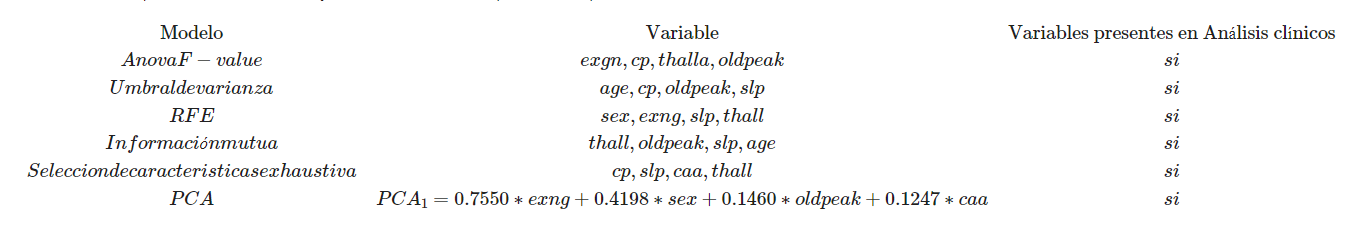
\includegraphics[width=0.60\textwidth]{feature_selection_cap4.png}
    \caption{Selección de características} 
    \label{fig:feature_selec}
\end{figure}


 La regresión lineal se puede representar mediante una ecuación lineal de la forma.

\begin{equation}
\hat{Y}_i = \hat{\beta}_0 + \hat{\beta}_1 X_i + \hat{\epsilon}_i
\end{equation}


Dado que nuestra variable de respuesta es una variable categórica se pretende que la línea forme un segmento discriminante en el cual una parte de los datos estén segmentado 2 por regiones las cuales se visualizaran por la línea ajustada.

Siguiendo el ejemplo de ecuación lineal anterior y basándonos en la figura \ref{fig:feature_selec} tenemos nuestra ecuación lineal.

\subsubsection{Comparacion con otros modelos}

El modelo ya mencionado se puede comparar con otros modelos que desempeñan otro tipo de características como Lasso Regression, este modelo usa un técnica de contracción, Contracción es donde los datos se encogen hacia un punto central de la media, Este tipo de modelos son muy utilizados cuando se muestran en nuestros datos un alto nivel de multicolinealidad o cuando la varianza en nuestros datos es muy grande. Otra de las ventajas de este modelo es su capacidad para la selección y eliminación de variables que aportan o no a nuestro modelo. Lasso Regression usa un tipo de técnica llamada regularización la cual es implementada al agregar un término llamada penalización la cual busca lograr la menor varianza en nuestro conjunto de datos de prueba.

\subsubsection{Métrica de evaluación}

Métrica de evaluación (Mean absolute error)
En el contexto de una regresión lineal, el error absoluto se refiere a la magnitud de la diferencia entre la predicción de una observación y el verdadero valor de la observación.
MAE toma el promedio de errores absolutos de un grupo de predicciones y observaciones como una medida de la magnitud de errores del grupo entero. Una de las propiedades que tiene esta métrica de evaluación es que es fácil de interpretar ya que el valor esta en la misma escala al valor que estamos realizando predicción.
Interpretación de MAE: su interpretación es simple ya que si su unidad esta mas cerca de el valor 0 mas preciso es el modelo.


\begin{equation}
\hat{Y}_i = \hat{\beta}_0 + \hat{\beta}_1 exng  + \hat{\beta}_2 cp  + \hat{\beta}_3 thalla  + \hat{\beta}_4 caa  + \hat{\beta}_5 thall + \hat{\epsilon}_i
\end{equation}


\subsection{Clasificación}
Los modelos de clasificación buscan predecir categorías a las que pertenece cierta etiqueta dados un conjunto de variables dependientes.
Para nuestro conjunto de datos los modelos de clasificación son la mejor opción ya que trataremos de predecir si cierto paciente presenta una enfermedad del corazón, Los modelos evaluados en esta sección fueron.

\begin{enumerate}
  \item SVM \emph{Support Vector Machine} \\
  SVM ha sido ampliamente utilizado como un poderoso método de machine learning en diferentes problemas de clasificación incluyendo bioinformatica. El modelo trata de buscar un óptimo hiper plano el cual maximice la distancia de el punto de datos de entrenamiento mas cercano. El hiper plano de el modelo SVM maximiza el margen mientras que minimiza el error de clasificación. El margen es computado como la suma de las distancias a unas de las mas cercanas positivas, sobre este modelo se encontró una optimización de un modelo para predecir ataques al corazón usando como base SVM \cite{8684835}.
  \item \emph{Random Forest classifier} \\
       El método \emph{Random Forest} es un estimador que ajusta diferentes arboles de clasificación en diferentes subconjuntos de el dataset y con el uso de la media para mejorar la predicción y controlar el sobre entrenamiento del modelo. este método fue elegido por trabajos previos con un buen despeño del modelo \cite{Pal_2021}.   
\end{enumerate}


\section{Adquisición de datos}
\label{sec:adquisiciondatos}

Dentro de este análisis el conjunto de datos es obtenido de UC Irvine \cite{UCI} , Los datos han sido recolectados de 303 pacientes de un subconjunto conjunto de datos que contiene 13 columnas y su variable de respuesta la cual es si el si el paciente presenta enfermedad del corazón o no. véase cuadro: \ref{table:comparative}.


\section{Resultados}

\subsection{Fuzzy C Means Clustering}
Se aplico el modelo FCM usando las 303 observaciones a fin de encontrar los mejores clústeres que representen nuestros datos.

\begin{figure}[ht]
    \centering
    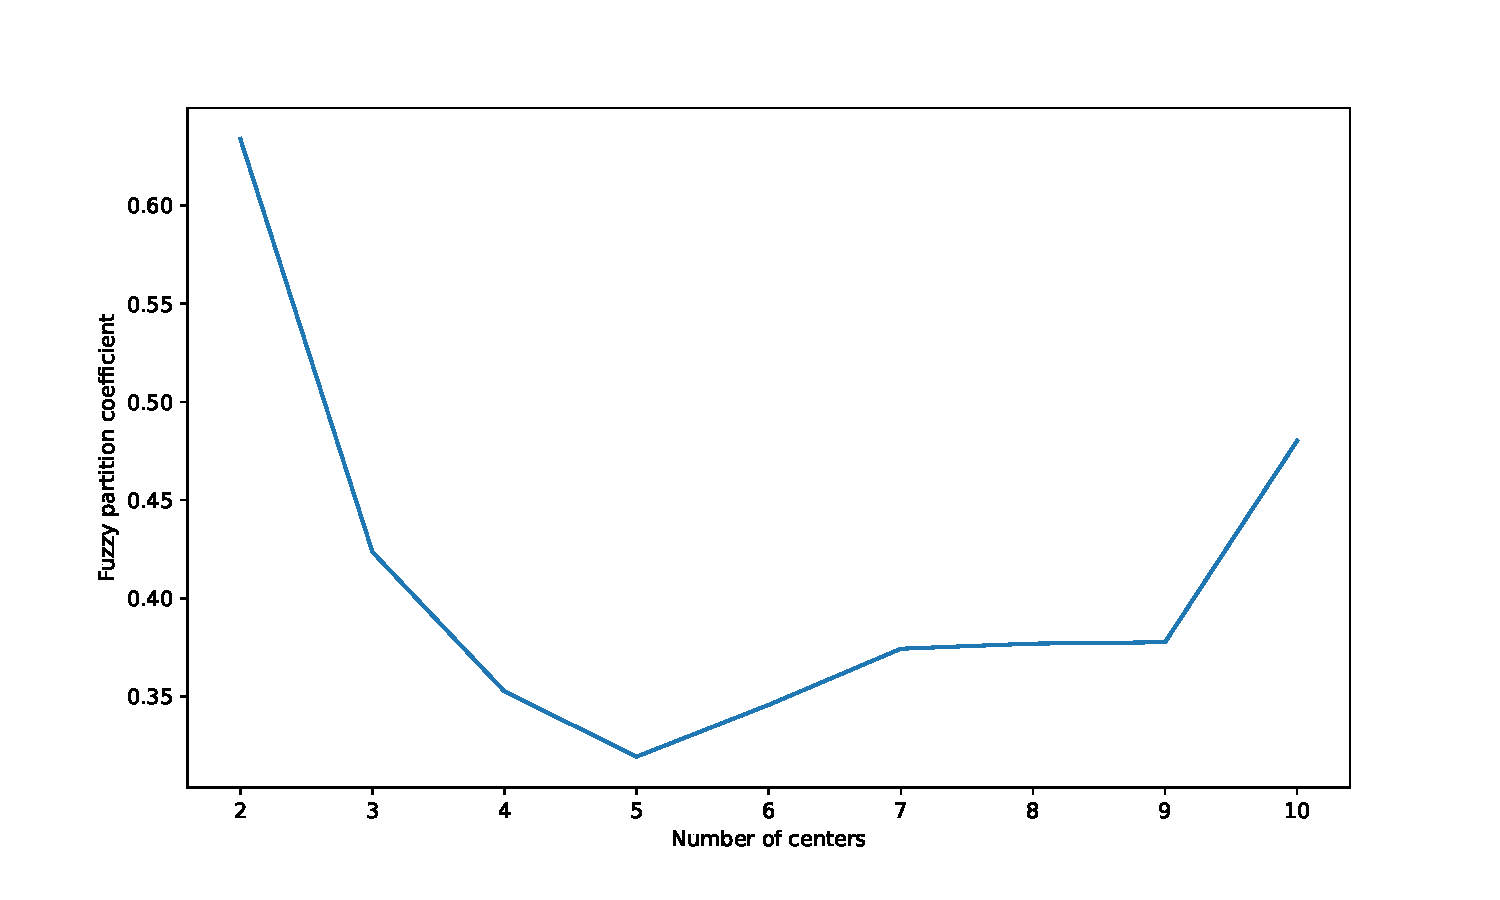
\includegraphics[width=0.5\textwidth,height=0.5\textheight,keepaspectratio]{elbow.pdf}
    \caption{ Grafica creada en el analisis de nuestro} 
    \label{fig:fcm_elbow}
\end{figure}

Los dados obtenidos en la métrica de evaluación fueron \textbf{2} clústeres como los óptimos en una iteración de 1 hasta 9 clústeres, representado claramente en con nuestra grafica de codo. \autoref{fig:fcm_elbow} La métrica de evaluación para este modelo fue su \textbf{coeficiente de particiones de fuzzy (FCP)} la cual marco un notable porcentaje en 2 clusters.


\subsection{Regresión Lineal}

Se aplico un modelo de regresión lineal el cual obtuvimos una regresión moderada usando nuestros datos, se considero aplicar un modelo de regresión simple ya que solo seleccionamos un conjunto de variables consideradas en el trabajo de selección de características \ref{fig:feature_selec}, con respecto a los resultados de  nuestra métrica de evaluación (MAE) se consideró  un valor muy bueno de  \textbf{0.29} lo cual nos habla de posibles iteraciones en modelos específicos a fin de incrementar nuestro valor de métrica usado.


\subsection{Clasificación}

Se aplicaron 2 modelos de clasificación de los cuales se encontró trabajos relacionados con predicción de ataques al corazón para nuestro conjunto de datos se aplico un preprocesa-miento usando PCA tomando solo los 2 principales componentes y aplicándolos a cada uno de los modelos.


Los resultados de los modelos fueron.

\begin{table}[th]
    \caption{Modelo usado y porcentaje de precisión.}
    \label{tab:ts_example}
    \begin{center}
    \begin{tabular}{|r|l|}
    \hline
       Modelo & Precisión  \\
   \hline
    \emph{SVM classifier} &  88.52\verb|%|  \\

    \hline
    \emph{Random Forest classifier} &  85.24\verb|%|  \\
   \hline
    \end{tabular}
    \end{center}
\end{table}

Dada la precision de los modelo podemos observar que el modelo SVM tuvo una mejor precision.


\section{Discusión}

\subsection{Fuzzy C Means Clustering}

Se observo un buen desempeño con respecto a el calculo del mejor número de clústeres siendo de 300ms aproximadamente sin la funcionalidad del multithreading. Los valores de las métricas que usa el modelo FCM nos permitió claramente ver el número de clústeres.  Una de las comparaciones a realizar a futuro seria comparar con un algoritmo tradicional tal como K-Means o K-Mediods a fin de comparar tiempo y si es tan notable el encuentro del mejor clúster.

\subsection{Linear Regression}


Se observo un buen desempeño usando un modelo de regresión simple usando ciertas características de nuestro conjunto de datos, la única parte que seria una parte de análisis es saber si usando mas características con modelos que discriminan y realizar una selección de características obtenemos mejores resultados o al menos saber si nuestro subconjunto de datos es el óptimo para nuestro modelo que se ejecutó.



\begin{table}[th]
\centering
\caption{Descripción de las 13 variables dentro del dataset usado en los modelos}\label{table:comparative}

\resizebox{0.5\textwidth}{!}{%
\begin{tabular}{p{1.2cm} c c c p{2cm} c c }\hline
\toprule
\textbf{Variable} & \textbf{Condición} & \textbf{Identificación}\\\hline
\midrule

\multirow{1}{2cm}{Sex} & \multirow{1}{0.95cm}{Gender} & Male/Female\\\hline

Age & Age of pacient & 20-90 \\ \hline

\multirow{4}{2cm}{cp} & \multirow{4}{2cm}{Tipo de dolor de pecho}  & 0 : Angina tipica  \\
 & & 1: Angina atipica  \\ & &    2: non-anginal pain \\ & &  3: asintomático
  \\\hline

 
trtbps & Azucar en ayunas > 120 & 290  \\ \hline

chol & Colesterol en mg dl & valor numerico \\\hline

\multirow{4}{3cm}{rest ecg} & \multirow{4}{4cm}{Resultado electrocardiograma en reposo}  & 0 : normal  \\
 & & 1:ST-T wave abnormality  \\ & &    2: ventricular hypertrophy by Estes criteria
  \\\hline

thalach & maximum heart rate achieved & valor numerico\\\hline

\multirow{2}{2cm}{exang} & \multirow{2}{2cm}{Angina de Pecho Inducida} & 1:Yes \\ & & 0: No  \\\hline

old peak & ST depression induced by exercise & valor numerico \\\hline

\multirow{2}{2cm}{slp} & \multirow{2}{2cm}{slope peak ST segment} & 0 = unsloping \\ & & 1 = flat \\ & & 2 = downsloping\\\hline


caa & number of major vessels &  0-3 \\\hline




\multirow{2}{2cm}{thall } & \multirow{2}{2cm}{thalassemia} & 0 = null \\ & & 1 = fixed defect \\ & & 2 = normal \\ & & 3 = reversable defect\\\hline



\bottomrule
\end{tabular}%
}
\begin{quote}
\scriptsize
\centering
$^{\dagger}$ 
\end{quote}
\end{table}

 

% Can use something like this to put references on a page
% by themselves when using endfloat and the captionsoff option.
\ifCLASSOPTIONcaptionsoff
  \newpage
\fi



% trigger a \newpage just before the given reference
% number - used to balance the columns on the last page
% adjust value as needed - may need to be readjusted if
% the document is modified later
%\IEEEtriggeratref{8}
% The "triggered" command can be changed if desired:
%\IEEEtriggercmd{\enlargethispage{-5in}}

% references section

% can use a bibliography generated by BibTeX as a .bbl file
% BibTeX documentation can be easily obtained at:
% http://mirror.ctan.org/biblio/bibtex/contrib/doc/
% The IEEEtran BibTeX style support page is at:
% http://www.michaelshell.org/tex/ieeetran/bibtex/

\bibliographystyle{IEEEtranN}
% argument is your BibTeX string definitions and bibliography database(s)
\nocite{articlePredictingFuzzyCMeans}
\nocite{articlePredictingFuzzyCMeans}
\nocite{inbookClusteringAndAsociationRules}
\nocite{fusterbarcel_2023_unleashing}
\nocite{emmanuelramos143FeatureSelection}
\nocite{stephenallwright_2022}
\bibliography{patient-id}
%
% <OR> manually copy in the resultant .bbl file
% set second argument of \begin to the number of references
% (used to reserve space for the reference number labels box)
%\begin{thebibliography}{1}

%\bibitem{IEEEhowto:kopka}
%H.~Kopka and P.~W. Daly, \emph{A Guide to {\LaTeX}}, 3rd~ed.\hskip 1em plus
%  0.5em minus 0.4em\relax Harlow, England: Addison-Wesley, 1999.

%\end{thebibliography}

% biography section
% 
% If you have an EPS/PDF photo (graphicx package needed) extra braces are
% needed around the contents of the optional argument to biography to prevent
% the LaTeX parser from getting confused when it sees the complicated
% \includegraphics command within an optional argument. (You could create
% your own custom macro containing the \includegraphics command to make things
% simpler here.)
%\begin{IEEEbiography}[{\includegraphics[width=1in,height=1.25in,clip,keepaspectratio]{mshell}}]{Michael Shell}
% or if you just want to reserve a space for a photo:

%\begin{IEEEbiography}{Michael Shell}
%Biography text here.
%\end{IEEEbiography}

% if you will not have a photo at all:
%\begin{IEEEbiographynophoto}{John Doe}
%Biography text here.
%\end{IEEEbiographynophoto}

% insert where needed to balance the two columns on the last page with
% biographies
%\newpage

%\begin{IEEEbiographynophoto}{Jane Doe}
%Biography text here.
%\end{IEEEbiographynophoto}

% You can push biographies down or up by placing
% a \vfill before or after them. The appropriate
% use of \vfill depends on what kind of text is
% on the last page and whether or not the columns
% are being equalized.

%\vfill

% Can be used to pull up biographies so that the bottom of the last one
% is flush with the other column.
%\enlargethispage{-5in}



% that's all folks
\end{document}


